\documentclass[12pt]{article}

% ── Packages ────────────────────────────────────────────────────────
\usepackage[margin=1in]{geometry}
\usepackage{amsmath,amssymb}
\usepackage{graphicx}
\usepackage{caption}
\usepackage{subcaption}
\usepackage{float}
\usepackage{placeins}
\usepackage{array}
\usepackage{tabularx}
\usepackage{setspace}         % Double spacing for Nature initial submission
\usepackage{lineno}           % Line numbers for peer review
\usepackage[numbers,sort&compress]{natbib} % Numbered refs for Nature style
\usepackage{xr-hyper}         % Must be loaded BEFORE hyperref
\usepackage{hyperref}
\hypersetup{colorlinks=true,linkcolor=blue,citecolor=blue,urlcolor=blue}

% Cross-document references to Supplementary Materials.
\IfFileExists{supplementary.aux}{%
  \externaldocument{supplementary}%
}{}

% Fallback: hardcoded supplementary labels so refs resolve even without aux.
\makeatletter
\AtBeginDocument{%
  \@ifundefined{r@fig:supp:signed-vs-abs-q}{\newlabel{fig:supp:signed-vs-abs-q}{{S1}{}}}{}%
  \@ifundefined{r@fig:supp:tau-ratio}{\newlabel{fig:supp:tau-ratio}{{S2}{}}}{}%
  \@ifundefined{r@fig:supp:binder-fss}{\newlabel{fig:supp:binder-fss}{{S3}{}}}{}%
  \@ifundefined{r@fig:supp:susceptibility-fss}{\newlabel{fig:supp:susceptibility-fss}{{S4}{}}}{}%
  \@ifundefined{r@fig:supp:ews-ac-var}{\newlabel{fig:supp:ews-ac-var}{{S5}{}}}{}%
  \@ifundefined{r@fig:supp:abm-multilag-ac}{\newlabel{fig:supp:abm-multilag-ac}{{S6}{}}}{}%
  \@ifundefined{r@fig:supp:symmetric-diagonal}{\newlabel{fig:supp:symmetric-diagonal}{{S7}{}}}{}%
  \@ifundefined{r@fig:supp:k-effect-split}{\newlabel{fig:supp:k-effect-split}{{S8}{}}}{}%
  \@ifundefined{r@fig:supp:k500-finite-size}{\newlabel{fig:supp:k500-finite-size}{{S9}{}}}{}%
  \@ifundefined{r@fig:supp:beta-branch-bias}{\newlabel{fig:supp:beta-branch-bias}{{S10}{}}}{}%
  \@ifundefined{r@fig:supp:beta-q-a}{\newlabel{fig:supp:beta-q-a}{{S11}{}}}{}%
  \@ifundefined{r@fig:supp:param-importance}{\newlabel{fig:supp:param-importance}{{S12}{}}}{}%
  \@ifundefined{r@fig:supp:time-series-overview}{\newlabel{fig:supp:time-series-overview}{{S13}{}}}{}%
  \@ifundefined{r@fig:supp:scatter-h1-h2}{\newlabel{fig:supp:scatter-h1-h2}{{S14}{}}}{}%
  \@ifundefined{r@fig:supp:eventstudy-h4}{\newlabel{fig:supp:eventstudy-h4}{{S15}{}}}{}%
  \@ifundefined{r@fig:supp:h2-density-12h}{\newlabel{fig:supp:h2-density-12h}{{S16}{}}}{}%
}
\makeatother

\newcolumntype{Y}{>{\raggedright\arraybackslash}X}
\newcolumntype{C}{>{\centering\arraybackslash}X}
\captionsetup[subfigure]{labelformat=empty,skip=0pt}

% ── Document ────────────────────────────────────────────────────────
\begin{document}
\doublespacing
\linenumbers

% ── Title ───────────────────────────────────────────────────────────
% Keep \author{} minimal: only names with superscripts.
% Affiliations are placed after \maketitle to avoid truncation
% in LaTeX's centered author block.
\title{\Large\textbf{Competing feedback channels drive phase transitions in collective emotion}}

\author{
  Jinlin Wu$^{1,*}$,\quad Zhihang Liu$^{2,*}$
}

\date{}
\maketitle

% ── Affiliations (placed after \maketitle for proper line-wrapping) ──
\begin{singlespace}
\noindent
{\small
$^{1}$Urban Governance and Design Thrust, The Hong Kong University of Science and Technology (Guangzhou), Guangzhou 511400, China\\[2pt]
$^{2}$Institute of Space and Earth Information Science, The Chinese University of Hong Kong, Shatin, Hong Kong, China\\[6pt]
$^{*}$Correspondence:\;
\href{mailto:jwu923@connect.hkust-gz.edu.cn}{jwu923@connect.hkust-gz.edu.cn} (J.W.),\;
\href{mailto:zhihangliu@cuhk.edu.hk}{zhihangliu@cuhk.edu.hk} (Z.L.)
}
\end{singlespace}

\vspace{1em}

% ── Abstract ────────────────────────────────────────────────────────
\begin{abstract}
\noindent
Collective emotional states on social media can persist near neutrality for extended periods and then shift abruptly into self-sustaining polarization, yet predicting when such transitions will occur remains an open computational challenge. We develop a computational framework that formalizes the competition between stabilizing mainstream media and amplifying user-generated media as a mixed-feedback dynamical system governed by a single control parameter---the channel-balance ratio. Mean-field analysis identifies a critical threshold beyond which the neutral state destabilizes through a pitchfork bifurcation, and a Ginzburg--Landau reduction yields a quartic effective potential whose landscape shifts from a single well to a double well as amplification dominates. A direction--intensity decomposition separates symmetry breaking from moderate-buffer depletion, providing a computable early-warning indicator: elevated engagement activity precedes polarization jumps. Agent-based simulations on Erd\H{o}s--R\'enyi and Barab\'asi--Albert networks confirm that the transition structure persists under finite-size fluctuations and heterogeneous connectivity. In large-scale social-media data from the COVID-19 period, both predicted signatures appear: segments with elevated activity exhibit larger polarization jumps, and greater user-generated dominance covaries with higher volatility. The framework provides a mechanistic, computationally tractable account of collective fragility and offers actionable early-warning diagnostics for platform governance.
\end{abstract}

% ════════════════════════════════════════════════════════════════════
\section{Introduction}
\label{sec:introduction}
% ════════════════════════════════════════════════════════════════════

Understanding how millions of individuals collectively shift from calm to polarized is a defining challenge for computational social science. Online platforms generate continuous streams of behavioral data---posts, shares, emotional expressions---that make collective sentiment observable at unprecedented resolution. Despite this observational richness, predicting when collective emotion will destabilize and identifying the structural conditions that govern system resilience remain open problems.

Existing computational work has addressed this problem from several directions. Agent-based models of opinion dynamics---including threshold and cascade models~\cite{Granovetter1978,CentolaMacy2007,WattsDodds2007,Nyborg2016}, voter and bounded-confidence dynamics~\cite{HolleyLiggett1975,SoodRedner2005,Deffuant2000,HegselmannKrause2002}, and contagion on complex networks~\cite{Centola2010,Centola2018Tipping,Iacopini2019,PastorSatorras2015}---have revealed how local interaction rules produce emergent consensus, fragmentation, or coexistence. Network-science methods have quantified how degree heterogeneity, clustering, and community structure shape diffusion and polarization~\cite{Watts2002,Dandekar2013,McPherson2001}. Natural language processing and deep learning enable large-scale sentiment classification that transforms raw text into time-resolved emotional signals~\cite{Brady2023,Kramer2014,Fan2014}. And data-driven analyses of information cascades have documented echo-chamber effects and algorithmic amplification on real platforms~\cite{Bakshy2015,DelVicario2016SciRep,DelVicario2016PNAS,Vosoughi2018,Cinelli2021}.

Despite these advances, a critical gap remains at the intersection of modeling and measurement. Existing computational models typically assume a \emph{single} information channel---local neighbors, a global field, or an external signal---and derive transitions from nonlinearity in agents' responses to that channel. Real information environments, however, are \emph{mixed ecologies}: stabilizing mainstream media coexist with amplifying user-generated content, and these channels exert opposing feedback on collective states~\cite{Chadwick2017,Tornberg2022,Piao2023}. Mainstream sources tend to counteract extreme sentiment (negative feedback), while user-generated content---amplified by attention-driven algorithms---reinforces the dominant direction (positive feedback)~\cite{DelVicario2016SciRep,Vosoughi2018}. This competition introduces a natural control parameter---the relative weight of amplifying versus stabilizing sources---but no existing computational framework formalizes this channel-balance competition or derives the transition structure it induces.

We address this gap with a computational framework that integrates analytical theory, agent-based simulation, and empirical validation. We model individuals as occupying three arousal states (high, medium, low) and sampling risk signals from a mixed environment that blends a stabilizing mainstream channel with an amplifying user-generated channel, controlled by a single parameter $r\in[0,1]$. Two macroscopic variables---polarization direction $q$ (net imbalance) and activity $a$ (engagement intensity, equivalently moderate-buffer depletion)---track the collective state. Mean-field analysis in the symmetric regime identifies a pitchfork bifurcation at a critical channel-balance $r_c$, and a Ginzburg--Landau reduction near criticality yields a quartic effective potential $V_{\mathrm{eff}}(q)=\tfrac{1}{2}\alpha q^{2}+\tfrac{u}{4}q^{4}$ with $\alpha\propto(r_c-r)$. A direction--intensity decomposition reveals that elevated activity---moderate-buffer depletion---serves as a computable early-warning indicator, because activity rises before a polarized direction is selected. Agent-based simulations on Erd\H{o}s--R\'enyi and Barab\'asi--Albert networks confirm that the transition structure persists under finite-size fluctuations and topological heterogeneity, with Binder cumulant crossings and critical slowing down providing finite-size diagnostics. In large-scale social-media data from the COVID-19 period, both predicted signatures appear: elevated activity precedes larger polarization jumps, and greater user-generated dominance covaries with higher volatility. Figure~\ref{fig:framework} summarizes this theory-to-data workflow.

\begin{figure}[H]
  \centering
  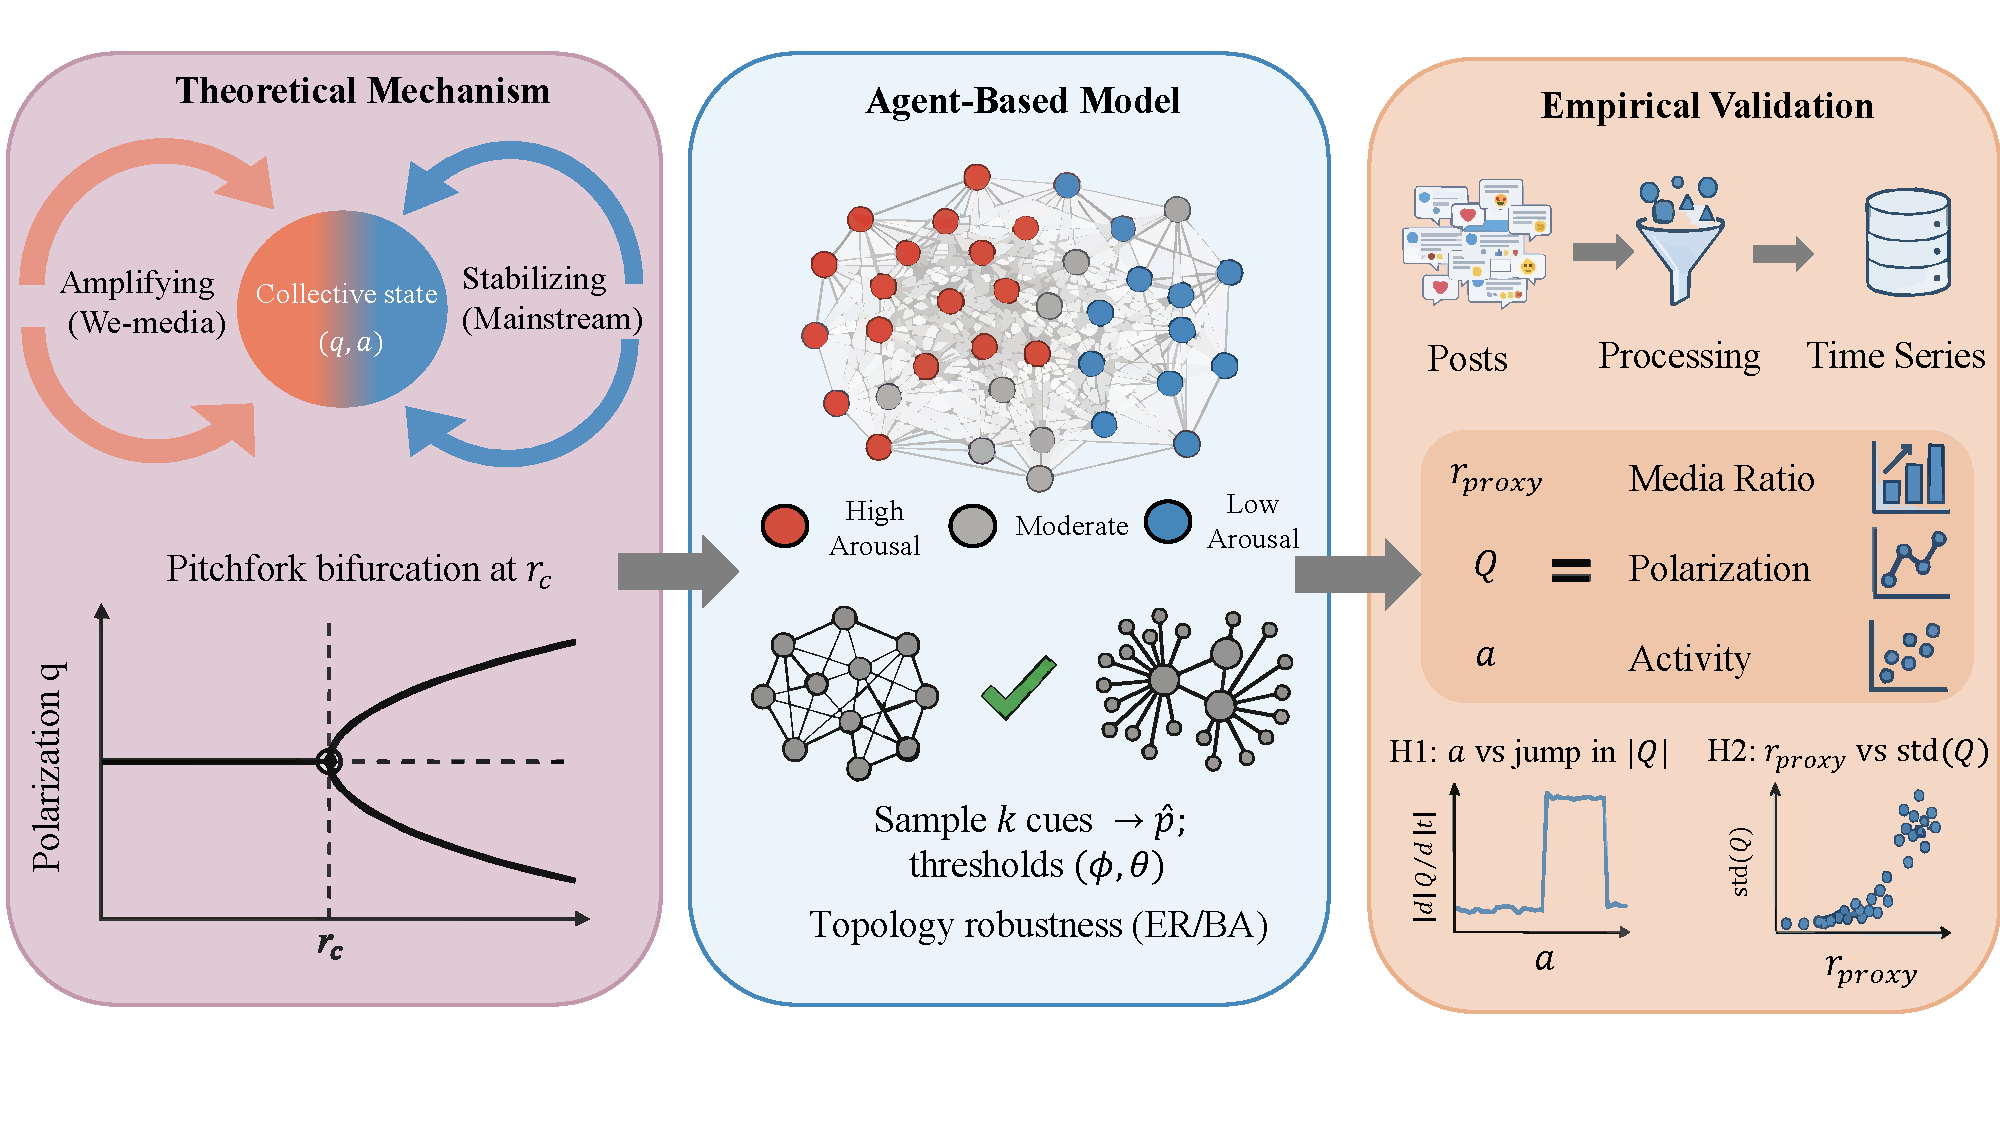
\includegraphics[width=0.95\linewidth]{figures/fig0_framework.pdf}
  \caption{\textbf{Computational framework overview.} (Left) Theory: a mixed-feedback model identifies a stability boundary and predicts bifurcation and activity-linked fragility. (Middle) Simulations: agent-based dynamics on networks confirm robustness beyond mean-field. (Right) Empirical tests: social-media time series are used to examine associations between activity, polarization jumps, and media composition.}
  \label{fig:framework}
\end{figure}

% ════════════════════════════════════════════════════════════════════
\section{Results}
\label{sec:results}
% ════════════════════════════════════════════════════════════════════
\noindent We present a theory-to-data evidence chain. Across mean-field analysis, network simulations, and empirical proxies, we show that mixed feedback yields a direction--intensity transition with bistability, that the parameter landscape identifies structural vulnerability conditions, and that two implied signatures---elevated activity predicting larger polarization jumps, and user-generated dominance covarying with higher volatility---appear in social-media data.

\subsection{Direction--intensity bifurcation}
\label{sec:direction-intensity-bifurcation}
Collective polarization is often attributed to external shocks, but competing media feedback can also generate endogenous instability when channel balance shifts. We characterize this mechanism by tracking two macroscopic variables: polarization direction $q$ (which side dominates) and activity $a$ (how heated the system is, i.e., depletion of the moderate buffer $\rho_M=1-a$). This separation matters because $a$ controls how much ``moderate mass'' remains to absorb perturbations: as $a\to 1$ the dynamics effectively reduce to two-state competition, increasing susceptibility to abrupt direction changes.

Mean-field analysis yields an analytic stability boundary. In the symmetric regime, linearizing around the neutral fixed point gives $dq/dt\approx(-1+\chi\Gamma)q$, where $\chi$ is the psychological sensitivity and $\Gamma$ is the feedback gradient of the mixed environment (Methods). The neutral state loses stability when $\chi\Gamma=1$, which yields the critical point
\begin{equation}
r_c=\frac{n_m(\chi+2)}{n_m(\chi+2)+n_w(\chi-2)}.
\label{eq:rc}
\end{equation}
For the baseline configuration (Methods), this gives $r_c\approx 0.753$. Near criticality, a Ginzburg--Landau reduction yields a quartic effective potential $V_{\text{eff}}(q)=\tfrac{1}{2}\alpha q^2+\tfrac{u}{4}q^4$ with $\alpha\propto(r_c-r)$, so the landscape shifts from a single well to a double well as stabilizing feedback is down-weighted. This bistability provides a mechanistic picture of polarized ``emotional bubbles'' as a loss of resilience (Fig.~\ref{fig:theory}a,b).

However, this clean bifurcation relies on a simplifying assumption: the user-generated channel responds symmetrically to positive and negative polarization. In realistic settings, attention-driven platforms tend to amplify whichever direction is already dominant, breaking this symmetry. To assess robustness, we compare the symmetric regime with an activity-coupled regime (Fig.~\ref{fig:theory}c).

Under symmetry, $|q|$ stays near zero until close to $r_c$ and $a$ rises mainly near the transition. Under activity-coupled asymmetry, direction and intensity become entangled: both $|q|$ and $a$ begin to increase already for $r<r_c$, turning the sharp tipping point into a broader crossover.

This direction--intensity entanglement has a crucial implication: elevated activity is not merely a symptom but a structural indicator of fragility. As stabilizing feedback weakens, the moderate buffer depletes (rising $a$), bringing the system closer to criticality even before a polarized direction is selected. Consistent with this, in asymmetric simulations activity relaxes faster than polarization ($\tau_a/\tau_q\approx 0.70$; Supplementary Fig.~\ref{fig:supp:tau-ratio}), indicating that $a$ must be tracked jointly with $q$. Such activity-leading patterns echo findings in online mobilization where recruitment surges precede collective alignment~\cite{GonzalezBailon2011,SteinertThrelkeld2015}.

\begin{figure}[H]
  \centering
  \begin{subfigure}[b]{0.48\linewidth}
    \centering
    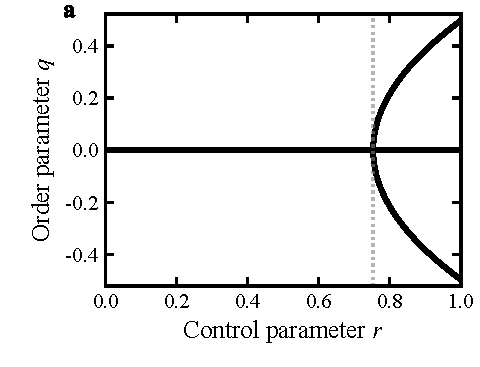
\includegraphics[width=\linewidth]{figures/fig1a_bifurcation.pdf}
    \caption{}
  \end{subfigure}
  \hfill
  \begin{subfigure}[b]{0.48\linewidth}
    \centering
    
\includegraphics[width=\linewidth]{figures/fig1b_potential.pdf}
    \caption{}
  \end{subfigure}
  \vspace{0.6em}
  \begin{subfigure}[b]{\linewidth}
    \centering
    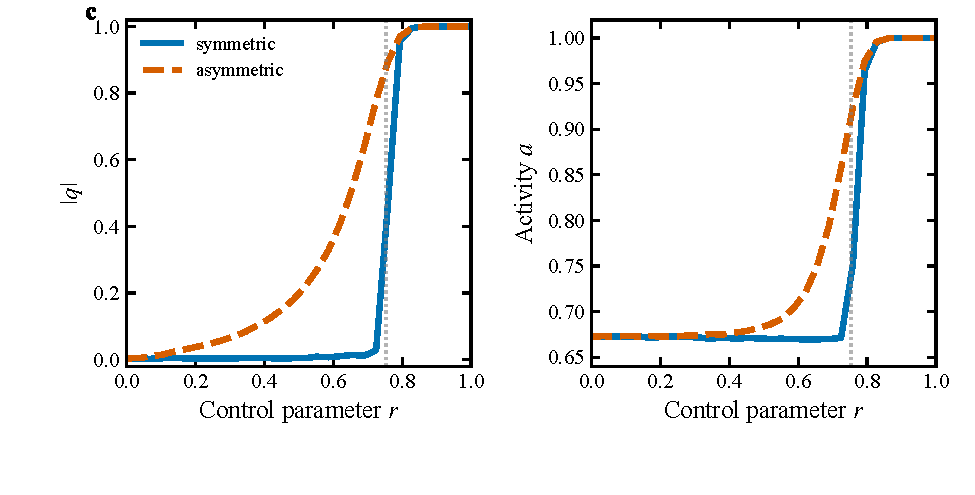
\includegraphics[width=\linewidth]{figures/fig1c_sym_asym_qa.pdf}
    \caption{}
  \end{subfigure}
  \caption{\textbf{Direction--intensity bifurcation.} \textbf{a}, Pitchfork bifurcation of the order parameter $q$ in the symmetric regime. \textbf{b}, Effective potential $V_{\mathrm{eff}}(q)$ for representative values of $r$ below, at, and above $r_c$; the inset magnifies the near-zero region. \textbf{c}, Steady-state $|q|$ (left) and activity $a$ (right) versus $r$ under symmetric and activity-coupled regimes; vertical dotted lines mark the theoretical $r_c$.}
  \label{fig:theory}
\end{figure}

\subsection{Bifurcation under networked interactions}
\label{sec:network-validation}
Network structure and finite-size fluctuations can blur or shift collective transitions, but they do not suppress the instability mechanism above. Real social systems are finite and networked; topology and stochasticity modulate where and how sharply macroscopic shifts appear. We examine networked dynamics by simulating microscopic updates on Erd\H{o}s--R\'enyi (ER) and Barab\'asi--Albert (BA) graphs across system sizes.

In the symmetric regime, networked agent-based dynamics retain the pitchfork transition. Trajectories select polarized branches with equal probability, so the signed mean $\langle Q\rangle$ cancels by symmetry; tracking $|Q|$ or aligning branch signs recovers the expected bifurcation (Fig.~\ref{fig:network_validation}a). Finite-size scaling is consistent with a transition: Binder cumulant curves $U_4(r;N)$---a standard finite-size diagnostic distinguishing phase transitions from crossovers---cross near the theoretical $r_c$ (Fig.~\ref{fig:network_validation}b), indicating that the estimated critical point is only weakly affected by finite-size corrections within our resolution. This crossing behavior is more stable than susceptibility peaks, which converge more slowly with system size (Supplementary Figs.~\ref{fig:supp:signed-vs-abs-q}--\ref{fig:supp:susceptibility-fss}).

Under activity-coupled asymmetry, the sharp bifurcation softens into a gradual crossover, while the qualitative shift persists across network topologies. Polarization $|Q|$ and activity $a$ rise together as user-generated dominance increases; under symmetry, activity rises mainly near $r_c$, whereas under activity-coupled asymmetry it increases earlier (Fig.~\ref{fig:network_validation}c). This direction--intensity coupling underlies the empirical activity--jump signature.

Across ER and BA topologies, networked dynamics preserve the central transition structure. Under symmetry, the pitchfork bifurcation remains sharp and $r_c$ stays close to the analytic boundary; under activity-coupled asymmetry, the transition becomes a crossover while direction--intensity coupling remains. This pattern mirrors a broader observation in network-mediated threshold dynamics: topology can modulate sharpness and location without removing collective transitions~\cite{Watts2002,Centola2010,Centola2018Tipping,Iacopini2019}.

\begin{figure}[H]
  \centering
  \begin{subfigure}[b]{0.48\linewidth}
    \centering
    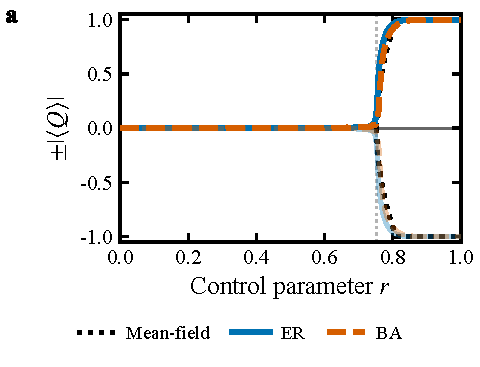
\includegraphics[width=\linewidth]{figures/fig2a_network_validation.pdf}
    \caption{}
  \end{subfigure}
  \hfill
  \begin{subfigure}[b]{0.48\linewidth}
    \centering
    
\includegraphics[width=\linewidth]{figures/fig2b_binder_u4.pdf}
    \caption{}
  \end{subfigure}
  \vspace{0.6em}
  \begin{subfigure}[b]{\linewidth}
    \centering
    
\includegraphics[width=\linewidth]{figures/fig2c_activity.pdf}
    \caption{}
  \end{subfigure}
  \caption{\textbf{Network robustness.} \textbf{a}, Steady-state polarization $|Q|$ versus $r$ in agent-based simulations on ER and BA networks; shaded bands denote 95\% confidence intervals across realizations. \textbf{b}, Binder cumulant $U_4(r;N)$ for multiple system sizes; the vertical dotted line marks the theoretical $r_c$. \textbf{c}, Steady-state polarization magnitude $|Q|$ and activity $a$ versus $r$ in agent-based simulations under symmetric (left) and activity-coupled (right) regimes; shaded bands denote 95\% confidence intervals across 50 seeds, and vertical dotted lines mark the theoretical $r_c$.}
  \label{fig:network_validation}
\end{figure}

\subsection{Parameter landscape}
\label{sec:parameter-landscape}
The bifurcation mechanism above is defined around a single baseline configuration; for practical prediction, we need to understand which systems are most vulnerable and what structural shifts can push a stable system toward criticality. The critical boundary $r_c$ is not universal. We map how it depends on four structural factors: psychological thresholds $(\phi,\theta)$, information density $k$, media ecology $n_w/n_m$, and local network coupling $\beta$ (Fig.~\ref{fig:landscape}).

Among these factors, media ecology is the most directly actionable. Increasing user-generated dominance (larger $n_w/n_m$) systematically lowers $r_c$ (Fig.~\ref{fig:landscape}c): when amplifying user-generated feedback outweighs stabilizing mainstream feedback, a smaller shift in the control parameter $r$ suffices to destabilize the neutral state. This mechanism aligns with empirical accounts of amplification and cocooning in online information environments~\cite{DelVicario2016SciRep,Piao2023}.

Psychological thresholds and information density shape vulnerability through the response sensitivity $\chi$. A transition exists only when $\chi>2$, defining a feasible region in the $(\phi,\theta)$ plane (Fig.~\ref{fig:landscape}a), with the baseline parameters lying inside this vulnerable zone. Increasing $k$ sharpens thresholded perception and typically amplifies responsiveness, but the induced shift in $r_c$ is non-monotonic (Fig.~\ref{fig:landscape}b), reflecting competing effects of enhanced sensitivity and reduced finite-sample variability in finite systems.
Moreover, media leverage depends on sensitivity: when $\chi$ is higher (e.g., at larger $k$), the same shift in $n_w/n_m$ produces a larger change in $r_c$, implying that high-sensitivity contexts are both more vulnerable and more responsive to structural interventions (Supplementary Fig.~\ref{fig:supp:param-importance}b).

Local coupling $\beta$ captures neighborhood reinforcement beyond the global environment. As $\beta$ increases, local reinforcement shifts the macroscopic boundary (Fig.~\ref{fig:landscape}d) and can bias branch selection, consistent with the general role of local reinforcement in threshold-based contagion~\cite{Granovetter1978,Centola2010,Iacopini2019}. These effects are robust across diagnostic checks (Supplementary Figs.~\ref{fig:supp:symmetric-diagonal}--\ref{fig:supp:beta-q-a}).

Sensitivity analysis confirms that media ecology and local coupling exert the largest effects on the stability boundary, each shifting $r_c$ by approximately two-thirds of its baseline value (Supplementary Fig.~\ref{fig:supp:param-importance}). These two factors are also the most actionable: media ecology can be adjusted via exposure mixing or algorithmic curation, while local coupling can be modulated by platform features that control neighbor-activity visibility. Psychological thresholds and information density, by contrast, act as contextual modifiers---high $\chi$ amplifies the leverage of structural interventions but is harder to change directly. The media-ecology effect motivates our empirical proxy $r_{\text{proxy}}$: if shifts toward user-generated dominance lower resilience in the model, they should manifest as increased volatility in real-world data.

\begin{figure}[H]
  \centering
  \begin{subfigure}[b]{0.48\linewidth}
    \centering
    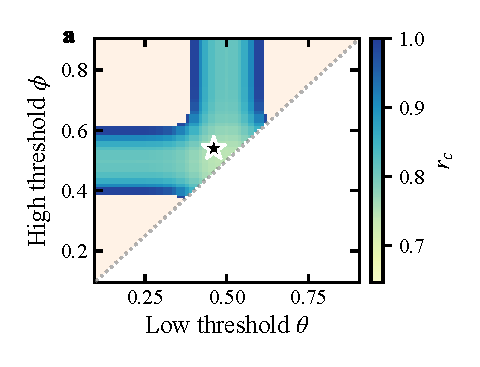
\includegraphics[width=\linewidth]{figures/fig4a_chi_rc_landscape.pdf}
    \caption{}
  \end{subfigure}
  \hfill
  \begin{subfigure}[b]{0.48\linewidth}
    \centering
    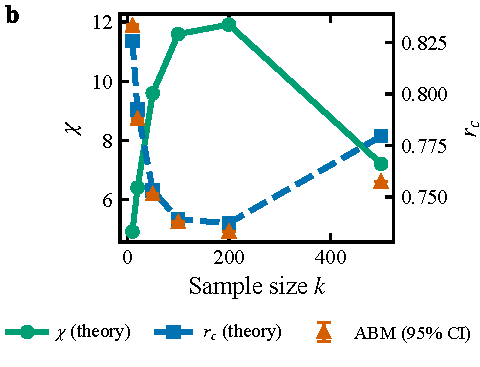
\includegraphics[width=\linewidth]{figures/fig4b_k_effect.pdf}
    \caption{}
  \end{subfigure}
  \vspace{0.5em}
  \begin{subfigure}[b]{0.48\linewidth}
    \centering
    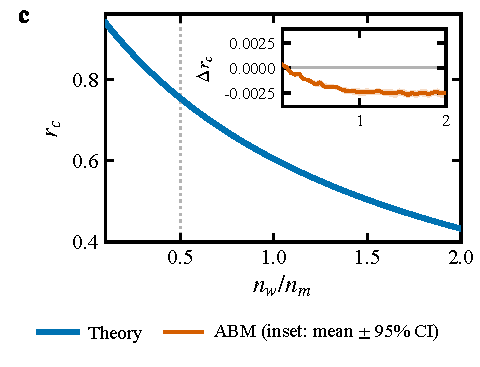
\includegraphics[width=\linewidth]{figures/fig4c_media_ratio.pdf}
    \caption{}
  \end{subfigure}
  \hfill
  \begin{subfigure}[b]{0.48\linewidth}
    \centering
    
\includegraphics[width=\linewidth]{figures/fig4d_beta_effect.pdf}
    \caption{}
  \end{subfigure}
  \caption{\textbf{Parameter landscape.} \textbf{a}, Critical point $r_c(\phi,\theta)$ in the symmetric regime; shaded: no transition ($\chi\le 2$); white: invalid ($\phi\le\theta$); star: baseline. \textbf{b}, Effect of information density $k$: psychological sensitivity $\chi$ (green, left axis) and critical point $r_c$ (blue theory and orange ABM with 95\% CIs, right axis). \textbf{c}, $r_c$ versus media ratio $n_w/n_m$ (gray dotted line: baseline; inset: $\Delta r_c=r_c^{\mathrm{ABM}}-r_c^{\mathrm{theory}}$ with ABM mean and 95\% CI). \textbf{d}, $r_c$ versus local coupling $\beta$; ABM estimates with 95\% CIs, and the gray dotted line denotes the theoretical $r_c$ at $\beta=0$.}
  \label{fig:landscape}
\end{figure}

\subsection{Critical slowing down}
\label{sec:critical-slowing-down}
Phase transitions leave dynamical fingerprints. As the system approaches criticality, restoring forces weaken: perturbations that would quickly decay far from the boundary persist longer near it. This critical slowing down is a canonical early-warning signal across complex systems~\cite{Wissel1984,Scheffer2009,Scheffer2012,Dakos2012,Lenton2012RSTA,Bury2021}. Our framework predicts the same signature: the relaxation time diverges as $\tau(r)\propto (r_c-r)^{-1}$ when approaching the critical point from below.

Mean-field dynamics confirm this scaling: in deterministic dynamics, perturbations around the stable fixed point relax exponentially with time constant $\tau$, and a log--log fit yields an exponent close to one (Fig.~\ref{fig:csd}a). As the effective potential $V_{\mathrm{eff}}(q)$ flattens before splitting into a double well, perturbations encounter weaker restoring forces and thus decay more slowly.

Agent-based simulations reproduce this slowing under network structure and finite-size fluctuations. Both the reduced SDE and the full ABM show rising autocorrelation as $r\to r_c$ (Fig.~\ref{fig:csd}b). The ABM exhibits near-zero autocorrelation far from criticality, where finite-size fluctuations decay rapidly, while the reduced SDE retains nonzero baseline autocorrelation under continuous stochastic forcing; in both cases autocorrelation increases as the system approaches $r_c$. Additional diagnostics---including variance trends and multi-lag autocorrelation checks---are consistent with this signature (Supplementary Figs.~\ref{fig:supp:ews-ac-var}--\ref{fig:supp:abm-multilag-ac}).

Representative steady-state trajectories provide an intuitive view: far from criticality fluctuations remain bounded, whereas near criticality excursions are larger and more persistent (Fig.~\ref{fig:csd}c). Critical slowing down thus provides a temporal complement to the static bifurcation boundary: autocorrelation rises before polarization emerges, offering a potential early-warning window.

\begin{figure}[H]
  \centering
  \begin{subfigure}[b]{0.48\linewidth}
    \centering
    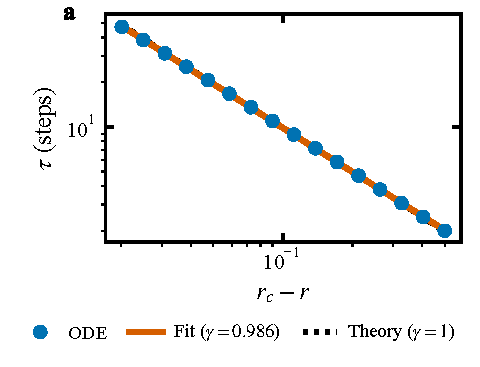
\includegraphics[width=\linewidth]{figures/fig3a_csd_scaling.pdf}
    \caption{}
  \end{subfigure}
  \hfill
  \begin{subfigure}[b]{0.48\linewidth}
    \centering
    
\includegraphics[width=\linewidth]{figures/fig3b_csd_sde_vs_abm.pdf}
    \caption{}
  \end{subfigure}
  \vspace{0.6em}
  \begin{subfigure}[b]{\linewidth}
    \centering
    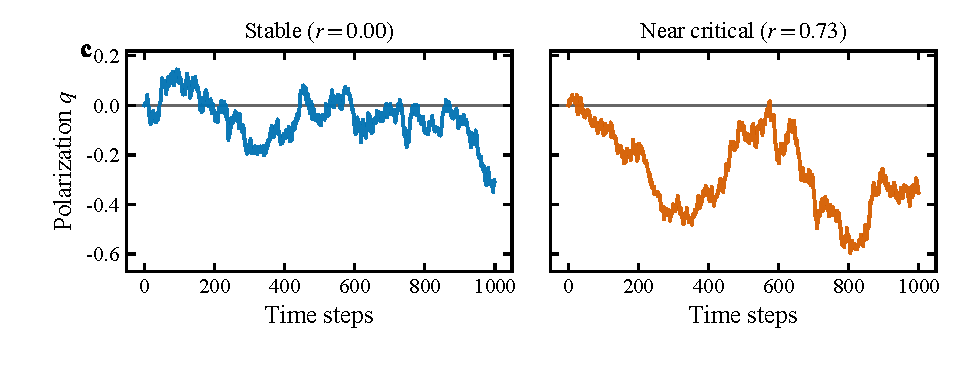
\includegraphics[width=\linewidth]{figures/fig3c_csd_timeseries.pdf}
    \caption{}
  \end{subfigure}
  \caption{\textbf{Critical slowing down as a dynamical signature.} \textbf{a}, Mean-field relaxation time $\tau$ versus distance to criticality $r_c-r$ for $r<r_c$. \textbf{b}, Lag-1 autocorrelation versus $r$ in the reduced SDE and the ABM; shaded bands denote 95\% confidence intervals, and the vertical dotted line marks the theoretical $r_c$. \textbf{c}, Representative steady-state trajectories far from and near the transition; fluctuations are larger and more persistent near criticality.}
  \label{fig:csd}
\end{figure}

\subsection{Empirical signatures in social-media data}
\label{sec:empirical-signatures}
The theory implies two observable signatures in social-media data. From the direction--intensity mechanism (Section~\ref{sec:direction-intensity-bifurcation}), segments with elevated activity exhibit larger polarization jumps (reflecting moderate-buffer depletion). From the parameter landscape (Section~\ref{sec:parameter-landscape}), greater user-generated dominance covaries with higher volatility (reflecting reduced resilience).

In the pooled dataset, segments with higher mean activity show larger jump intensity (95th percentile of $|d|Q|/dt|$; Pearson $r=0.241$, $p=0.00798$; Fig.~\ref{fig:empirical}a), linking moderate-buffer depletion to heightened susceptibility to abrupt direction changes.

User-generated dominance is positively associated with polarization volatility in the high-density subset (Pearson $r=0.429$, $p=6.03\times 10^{-7}$; Fig.~\ref{fig:empirical}b). The association is robust to controls for segment sampling density (Supplementary Fig.~\ref{fig:supp:h2-density-12h}), linking channel-balance shifts toward amplifying sources to reduced resilience.

Representative time series illustrate these patterns at the segment level: the high-activity segment exhibits larger polarization swings than its low-activity counterpart (Fig.~\ref{fig:empirical}c), and the high-$r_{\text{proxy}}$ segment shows greater fluctuation amplitude than the low-$r_{\text{proxy}}$ segment (Fig.~\ref{fig:empirical}d).

Together, these associations reveal two complementary dimensions of collective fragility. The activity--jump link (Fig.~\ref{fig:empirical}a,c) captures how the system \emph{approaches} instability: as the moderate buffer depletes, the remaining population becomes increasingly susceptible to abrupt directional shifts. The media-composition--volatility link (Fig.~\ref{fig:empirical}b,d) captures how information architecture \emph{sets} the resilience boundary: when amplifying channels dominate, even moderate perturbations produce larger fluctuations. Both signatures are consistent with the mixed-feedback mechanism: fragility emerges not from extreme content alone, but from structural conditions---depleted buffers and skewed channel balance---that erode the system's capacity to absorb shocks. Supplementary Figs.~\ref{fig:supp:scatter-h1-h2}--\ref{fig:supp:eventstudy-h4} report additional diagnostics across datasets and event-aligned analyses under realistic missingness.
\begin{figure}[H]
  \centering
  \begin{subfigure}[b]{0.48\linewidth}
    \centering
    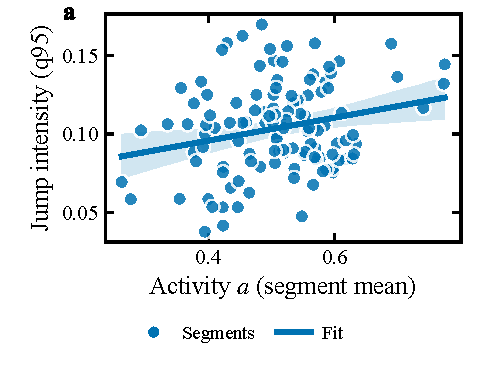
\includegraphics[width=\linewidth]{figures/fig5a_activity_jump.pdf}
    \caption{}
  \end{subfigure}
  \hfill
  \begin{subfigure}[b]{0.48\linewidth}
    \centering
    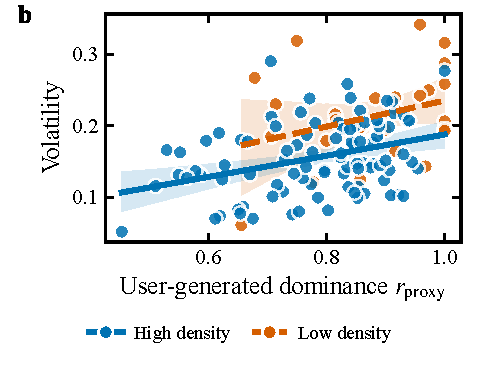
\includegraphics[width=\linewidth]{figures/fig5b_media_volatility_density.pdf}
    \caption{}
  \end{subfigure}
  \vspace{0.6em}
  \begin{subfigure}[b]{0.48\linewidth}
    \centering
    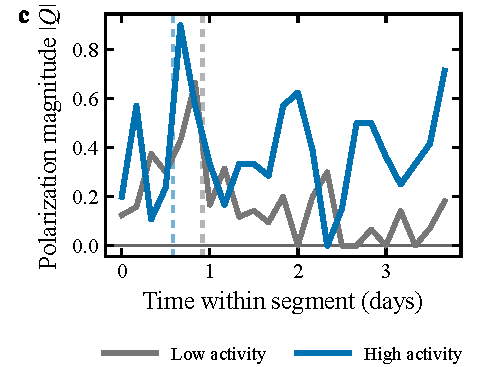
\includegraphics[width=\linewidth]{figures/fig5c_h1_example_timeseries.pdf}
    \caption{}
  \end{subfigure}
  \hfill
  \begin{subfigure}[b]{0.48\linewidth}
    \centering
    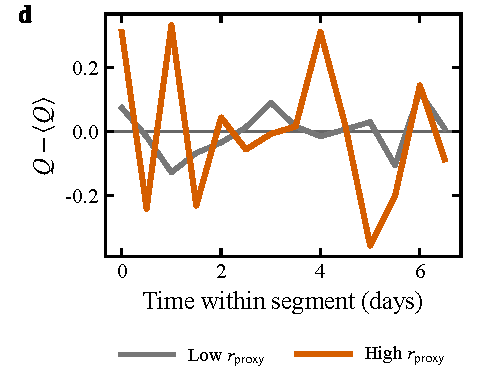
\includegraphics[width=\linewidth]{figures/fig5d_h2_example_timeseries.pdf}
    \caption{}
  \end{subfigure}
  \caption{\textbf{Empirical signatures at the segment level.} \textbf{a}, Activity $a$ versus jump intensity $\text{jump}_{q95}$ in the pooled dataset (see Methods for definitions). \textbf{b}, $r_{\text{proxy}}$ versus volatility in the high-density subset (12-hour aggregation); color indicates segment sampling density (median split). \textbf{c}, Representative high-activity (blue) and low-activity (gray) segments; vertical dashed lines mark the maximal single-step change in $|Q|$ within each segment. \textbf{d}, Representative high-$r_{\text{proxy}}$ (orange) and low-$r_{\text{proxy}}$ (gray) segments; $Q$ is shown after subtracting the segment mean to facilitate volatility comparison.}
  \label{fig:empirical}
\end{figure}

\begin{table}[H]
  \centering
  \caption{\textbf{Empirical tests of the two predicted signatures.} Partial correlation controls for segment sampling density.}
  \label{tab:empirical}
  \footnotesize
  \setlength{\tabcolsep}{4pt}
  \begin{tabularx}{\linewidth}{YCCCC}
    \hline
    Test & Dataset & Aggregation & Pearson $r$ ($p$) & Partial $r$ ($p$) \\
    \hline
    Activity $\to$ Jump intensity & Pooled & 4H & $r=0.241$ ($p=0.00798$) & -- \\
    $r_{\text{proxy}}\to$ Volatility & High-density & 12H & $r=0.429$ ($p=6.03\times 10^{-7}$) & $r=0.386$ ($p=8.79\times 10^{-6}$) \\
    \hline
  \end{tabularx}
\end{table}

\FloatBarrier

% ════════════════════════════════════════════════════════════════════
\section{Discussion}
\label{sec:discussion}
% ════════════════════════════════════════════════════════════════════

Our computational framework reveals that competition between feedback channels with opposite signs---stabilizing mainstream and amplifying user-generated media---produces a phase transition in collective emotional states, governed by a single control parameter that tunes channel balance. This mechanism is distinct from, and complementary to, existing computational models of collective transitions. Cascade and threshold models~\cite{Granovetter1978,Watts2002,CentolaMacy2007} typically require an external trigger to initiate a cascade; here, the transition arises endogenously as channel balance crosses a critical boundary. Bounded-confidence models~\cite{Deffuant2000,HegselmannKrause2002} produce fragmentation through tolerance narrowing; our model produces bifurcation through feedback competition. Echo-chamber accounts~\cite{Bakshy2015,DelVicario2016SciRep,DelVicario2016PNAS} emphasize selective exposure; our framework emphasizes state-dependent amplification, where the user-generated channel responds to both polarization and activity, yielding direction--intensity entanglement that selective-exposure models do not capture.

The direction--intensity decomposition offers a computational lens on collective fragility that complements existing social science perspectives. Conventional monitoring focuses on directional imbalance (which side is winning), but the activity variable $a$ captures a complementary dimension: how much moderate buffer remains. Because activity can rise while $q$ stays near zero, tracking engagement intensity alongside directional imbalance can provide earlier warning of approaching instability. This decomposition extends risk-amplification~\cite{Kasperson1988} and emotional-contagion~\cite{Kramer2014,Fan2014,Brady2023} perspectives by formally separating intensity from direction, and connects with hybrid media system analyses in which legacy and platform-native channels interact to shape collective response~\cite{Chadwick2017}.

The analytical tractability of the framework---critical point in closed form, Ginzburg--Landau reduction near criticality, and critical slowing down as a computable early-warning signal---offers practical tools for computational social science. The quartic potential provides a familiar landscape for understanding bistability and hysteresis, and the channel-balance ratio $r$ maps directly to measurable platform features. This analytical grounding complements the data-driven approaches that dominate computational studies of online polarization, providing a mechanistic bridge between platform design choices and collective outcomes.

Several practical implications follow. \textbf{Exposure mixing}---increasing the visibility of stabilizing sources during high-activity periods---could counteract amplification without removing content. \textbf{Activity monitoring} leverages direction--intensity coupling: elevated engagement, not only extreme content, can signal periods of heightened fragility. \textbf{Algorithmic damping}---reducing amplification gain on high-arousal content---lowers the effective channel balance and shifts the system away from criticality. These structural interventions complement content-level moderation and may be more scalable in high-volume environments.

Several limitations point to concrete extensions. The model treats sources within each channel as homogeneous; incorporating heterogeneity in credibility and audience size could clarify when a small number of influential accounts dominate feedback. Network structure in our simulations is limited to ER and BA graphs; real social networks feature homophily and community organization that can modulate polarization dynamics~\cite{McPherson2001,Dandekar2013}. Psychological thresholds are fixed population averages; incorporating threshold distributions may reshape both the stability boundary and precursor behavior~\cite{Schwartz2013,Pfefferbaum2020}. Empirically, $r_{\text{proxy}}$ is a count-based proxy rather than a measure of exposure, and connecting the framework to platform-side exposure metrics would provide more direct tests of media-ecology effects. Finally, extending the analysis to multiplex networks---where agents interact on multiple platforms simultaneously---and to time-varying channel balance could capture the co-evolutionary dynamics of media ecosystems.

\FloatBarrier

% ════════════════════════════════════════════════════════════════════
\section{Methods}
\label{sec:methods}
% ════════════════════════════════════════════════════════════════════
\noindent Our approach proceeds in four stages: we build a minimal mechanistic model of competing feedback channels, derive analytic conditions for the stability boundary, assess robustness and map parameter effects in network simulations, and confront the resulting signatures with empirical proxies. This sequence grounds the statistical tests in theoretically motivated signatures.

The model rests on three design choices: separating collective state into direction (which side dominates) and intensity (how heated the system is) to track moderate-buffer depletion separately from polarization; parameterizing the information environment as a mixture of stabilizing mainstream and amplifying user-generated channels controlled by $r$; and modeling individual responses as threshold-based transitions in response to sampled signals, yielding nonlinear feedback at the population level.

\subsection{Model framework}
We consider a population of $N$ individuals with three arousal states: high ($H$), medium ($M$), and low ($L$). Let $(\rho_H,\rho_M,\rho_L)$ denote the population fractions with $\rho_H+\rho_M+\rho_L=1$. To separate polarization direction from intensity, we introduce two macroscopic variables: the polarization direction
\begin{equation}
q(t)=\rho_H(t)-\rho_L(t),
\label{eq:q}
\end{equation}
and the system activity
\begin{equation}
a(t)=\rho_H(t)+\rho_L(t)=1-\rho_M(t).
\label{eq:a}
\end{equation}
Here, $q(t)$ measures which side dominates and $a(t)$ measures how heated the system is. These variables decouple symmetry breaking from the depletion of the moderate buffer $\rho_M=1-a$, with $\rho_H=(a+q)/2$ and $\rho_L=(a-q)/2$. When the buffer collapses ($a\to 1$), the dynamics effectively reduce to competition between extreme states.

At each update, an individual samples $k$ risk signals from the environment; each signal is labeled ``risk'' with probability $p_i$. Let $S\sim\text{Binomial}(k,p_i)$ denote the number of risk signals and $\hat{p}=S/k$ the perceived risk fraction. The individual transitions to $H$ if $\hat{p}\ge\phi$, to $L$ if $\hat{p}\le\theta$, and otherwise remains in $M$, where $\theta<\phi$ define low and high arousal thresholds.

The information environment is modeled as a competition between a stabilizing mainstream channel (negative feedback) and an amplifying user-generated channel (positive feedback). The mainstream signal is
\begin{equation}
p^{\text{main}}(q)=\frac{1-q}{2},
\label{eq:pmain}
\end{equation}
which counteracts the current polarization.

The user-generated channel, unlike mainstream media, can respond to the current collective state in multiple ways. To separate analytic tractability from empirical realism, we use two complementary formulations. The symmetric regime enforces directional symmetry ($q\to -q$) and enables closed-form derivation of the critical point. The activity-coupled regime allows amplification to depend on activity as well as direction, capturing attention-driven reinforcement observed on real platforms.

In the symmetric regime, we set
\begin{equation}
p^{\text{we}}(q)=\frac{1}{2}+\frac{q}{2},
\label{eq:pwe_sym}
\end{equation}
which enforces $q\to -q$ symmetry. In the activity-coupled regime we allow activity coupling via
\begin{equation}
p^{\text{we}}(q,a)=\rho_H=\frac{a+q}{2}.
\label{eq:pwe_asym}
\end{equation}
The overall environmental risk is the weighted average
\begin{equation}
p_{\text{env}}(q,a;r)=\frac{(1-r)n_m p^{\text{main}} + r n_w p^{\text{we}}}{(1-r)n_m + r n_w}, \qquad r\in[0,1],
\label{eq:penv}
\end{equation}
where $n_m$ and $n_w$ are the baseline strengths of the mainstream and user-generated channels, and the control parameter $r$ tunes their relative weight ($r=0$: mainstream-dominant; $r=1$: user-generated-dominant).

\subsection{Mean-field analysis and critical point}
Mean-field analysis characterizes when polarization becomes self-sustaining in the symmetric regime. The neutral state $q=0$ is a fixed point with $p_{\text{env}}=1/2$. We linearize the mean-field dynamics around this point and express stability in terms of two quantities: the psychological sensitivity $\chi$, measuring how strongly the collective response changes with environmental risk near neutrality, and the feedback gradient $\Gamma=\left.\partial p_{\text{env}}/\partial q\right|_{q=0}$, capturing how the mixed environment amplifies or damps polarization. The neutral fixed point loses stability when $\chi\Gamma$ exceeds unity (with $\chi\Gamma=1$ defining the stability boundary). Solving this condition yields an analytic critical point $r_c$ (reported in Results), and a Ginzburg--Landau reduction near criticality yields a quartic effective potential and predicts pitchfork bifurcation and critical slowing down. Full derivations are provided in Supplementary Materials S2.

\subsection{Agent-based network simulations}
We implement microscopic dynamics on Erd\H{o}s--R\'enyi (ER) and Barab\'asi--Albert (BA) networks with size $N$ and average degree $\langle k\rangle$~\cite{Erdos1959,Barabasi1999,PastorSatorras2015}. Updates are asynchronous: each step updates a fraction $f$ of nodes. We report time in steps and in sweeps, where one sweep corresponds to $N$ asynchronous updates (approximately $1/f$ steps). To capture local reinforcement, we introduce a coupling parameter $\beta$ that blends the global environment $p_{\text{env}}$ with neighbor information when forming each agent's perceived risk probability; $\beta=0$ recovers the well-mixed limit. Here $\langle k\rangle$ denotes average network degree, whereas $k$ denotes the number of sampled signals per update.

From node states we compute polarization $Q$ and activity $a$ using the same definitions as in Eqs.~(\ref{eq:q})--(\ref{eq:a}). In the symmetric regime, trajectories select either polarized branch with (approximately) equal probability, so the signed mean $\langle Q\rangle$ cancels by symmetry. We therefore track $|Q|$ or align trajectory signs across realizations before averaging.

Finite-size effects blur sharp transitions, so critical-point estimation can be sensitive to noise. To diagnose finite-size scaling in the baseline configuration, we use Binder cumulant crossings~\cite{Binder1981,NewmanBarkema1999}, which are more robust than susceptibility peaks:
\begin{equation}
U_4(r;N)=1-\frac{\langle Q^4\rangle}{3\langle Q^2\rangle^2}.
\label{eq:binder}
\end{equation}

To assess whether the critical-slowing-down signature predicted by mean-field theory is reproduced in simulations, we estimate relaxation time in deterministic mean-field dynamics and lag-1 autocorrelation of polarization trajectories in the reduced SDE and ABM. We report autocorrelation at lag 1 sweep after converting ABM steps to sweeps as above; additional diagnostics are provided in Supplementary Materials S4.

To map how structural parameters move the transition boundary, we vary information density $k$, media ratio $n_w/n_m$, and local coupling $\beta$ over broad ranges and estimate $r_c$ from the steepest slope of the median $|Q|(r)$ across seeds, with confidence intervals obtained by bootstrap. Specific parameter grids and estimation procedures are provided in Supplementary Materials S5.

\subsection{Empirical data and operational proxies}
We construct empirical proxies that map the direction--intensity variables to window- and segment-level observables.

We use a Weibo corpus spanning March 2020 to July 2025, covering the acute COVID-19 period and its longer aftermath, when public-health risk narratives remained salient. The corpus includes posts from mainstream media, government accounts, user-generated media accounts (``wemedia''), and public users. After de-duplication and filtering, we obtain 880,100 unique posts; the analyses reported here use an annotated subset of 90,982 posts.

Each post is annotated for emotional arousal (High/Medium/Low) and risk content (risk/norisk) using \texttt{Qwen3-8B}~\cite{Qwen3_8B} with structured prompts (Supplementary Materials S1). On a manually rated subset ($n=5{,}000$), the LLM achieved 85\% exact-match accuracy for arousal labels (Cohen's $\kappa=0.79$) and 87\% exact-match accuracy for risk labels ($\kappa=0.82$) (Supplementary Materials S1).

We aggregate posts into time windows and compute window-level proxies (4-hour windows in the primary analysis; 12-hour windows for robustness checks of media-composition estimates). Within each window, we compute arousal fractions $(X_H,X_M,X_L)$ from public-user posts; windows with fewer than 5 public posts are treated as missing. We compute media-type counts from all posts. We then construct polarization $Q=X_H-X_L$ and activity $a=X_H+X_L$. Media composition is proxied by
\begin{equation}
r_{\text{proxy}}=\frac{n_{\text{wemedia}}}{n_{\text{wemedia}}+n_{\text{mainstream}}+n_{\text{government}}},
\label{eq:rproxy}
\end{equation}
treating government accounts as part of the mainstream channel because they typically share the stabilizing orientation of official narratives during public crises.

For segment-level analyses, we group consecutive windows into weekly segments and retain those with sufficient coverage (at least 10 valid windows for $Q$ and $a$, and at least 5 valid consecutive differences for derivative-based statistics). Within each retained segment, volatility is $\text{std}(Q)$ and jump intensity is $\text{jump}_{q95}$, the 95th percentile of $|d|Q|/dt|$ computed on consecutive windows. Dataset definitions (pooled and high-density subsets) and robustness diagnostics are provided in Supplementary Materials S6.

\subsection{Code and data availability}
All simulation code, analysis scripts, and aggregated data are available at \url{https://github.com/[anonymized-for-review]} and will be deposited in a public repository with a DOI upon acceptance. The raw Weibo corpus is subject to platform terms of service; anonymized and aggregated data are available from the corresponding authors upon reasonable request.

\FloatBarrier

% ── End matter ──────────────────────────────────────────────────────

\section*{Author contributions}
J.W. conceived the study, developed the computational framework, performed analyses, and wrote the manuscript.
Z.L. co-conceived the study, developed the computational framework, supervised the project, and reviewed the manuscript.

\section*{Competing interests}
The authors declare no competing interests.

\section*{Acknowledgements}
This work was supported by the National Natural Science Foundation of China.

\bibliographystyle{unsrtnat}
\bibliography{references}

\end{document}
